%% Document class (Koma Script) -----------------------------------------
\documentclass[%
   %draft,						% under-/overfull boxes are marked with black square, no pictures
   final,							% final document
%%%% === Font Size ===
   11pt,
%%%% === Language ===
   ngerman,						% delegated to other packages
%%%% === Page Size ===
   % letterpaper,
   % legalpaper,
   % executivepaper,
   a4paper,
   % a5paper,
   % landscap,
%%%% === Options for type area ===
   BCOR1cm,						% Binding correction offset
   DIV11,							% Page Size (see Koma script documentation!)
   DIV=calc,					% automatic line length calculation
   1.1headlines,			% Line count for head
   %headinclude,			% include head into calculations
   headinclude=false,	% exclude head from calculations
   footinclude=false,	% exclude foot from calculations
   mpinclude=false,		% exclude margin from calculations
   pagesize,					% write page size to document file
											% Important for correct size conversions
%%%% === Layout ===
   oneside,						% one-side layout
   %twoside,					% side margins for two-side layout
   onecolumn,					% single column layout
   %twocolumn,				% double column layout
   %openany,         	% chapters may start on any page
   openright,					% chapters may only start on a right side (unimportant for oneside layouts)
	 headings=big,			% choices: small, normal, big
   										% print headings in appendix like others
   										% onelineappendix, noappendixprefix, appendixwithoutprefix, appendixwithoutprefixline
   										% print chapter headings like others
   										% onelinechapter, nochapterprefix, chapterwithoutprefix, chapterwithoutprefixline
   										% print headings in appendix with additional prefix line
   										% twolineappendix, appendixprefix, appendixwithprefix, appendixwithprefixline
   										% print headings in chapter with additional prefix line
   										% twolinechapter, chapterprefix, chapterwithprefix, chapterwithprefixline
   										% openany: \clearpage not \cleardoublepage after chapters, index, etc.
   										% openleft: \clear-commands may produce page break & start chapter on left page
   										% openright: \clear-commands may produce page break & start chapter on right page
   										%
   captions=oneline,	% seperate handling of one-line captions --> centered
	 %captions=nooneline,% no seperate handling of one-line captions
	 %captions=heading,	% captions of floating environments are formatted as headings, placement dependent on
	 										% \caption{} position!, equal to above & top, implicate captions=tableheading|figureheading
	 %captions=signature,	% captions of floating environments are formatted as headings, placement dependent on
	 										% \caption{} position!, equal to above & top, implicates captions=tablesignature|figuresignature
	 %captions=figureheading,	% figures will have their caption 'on top', equal to figureabove, abovefigure,
	 													% topatfigure, typographically undesirable!
	 %captions=figuresignature	% figures will have a trailing caption, equal to belowfigure, bottomatfigure
	 													% this is what you want! (caption will be formatted as captionbelow)
	 captions=tableheading,		% tables will have their caption 'on top', equal to tableabove, abovetable,
	 													% abovetabular, topattable, this is what you want! (caption will be formatted as captionabove)
	 %captions=tablesignature	% tables will have a trailing caption, equal to belowtable, belowtabular, bottomattable
	 										%
	 										% other caption options: topbeside, bottombeside, centeredbeside, innerbeside, outerbeside,
	 										%	leftbeside, rightbeside
   cleardoublepage=plain,	% empty left side mit page style 'plain'
   %cleardoublepage=empty,	% empty left side mit page style 'empty'
   titlepage,					% title as standalone page ('titlepage' environment)
   %notitlepage,			% title integrate in other page
%%%% --- Paragraph Indentation ---
   %									% Paragraph spacing: single-spaced
   parskip=true,			% options:
   										% full|true|on|yes: paragraphs denoted by 1 line vertical spacing, no indentation
   										% full-						: paragraphs denoted by 1 line vert. spacing, ends undenoted
   										% full+						: paragraphs denoted by 1 line vert. spacing, ends with third of a line spacing
   										% full*						: paragraphs denoted by 1 line vert. spacing, ends with quarter of a line spacing
   										% half						: paragraphs denoted by 1/2 line vert. spacing, ends with third of a line spacing
   										% half-						: paragraphs denoted by 1/2 line vert. spacing, ends undenoted
   										% half+						: paragraphs denoted by 1/2 line vert. spacing, ends with third of a line spacing
   										% half*						: paragraphs denoted by 1/2 line vert. spacing, ends with quarter of a line spacing
   										% false|off|no		: paragraphs denoted by indentation
   										% never						: no spacing between paragraphs
%%%% === Header ===
%
   headsepline=true,	% line below header
   footsepline=false,	% no line above footer
%
%%%% === Lists (TOC, LOF, LOT, BIB) ===
%
   toc=bibliography,	% include bibliography in table of contents unnumbered
   										% alternatives:	bib, bibliographynumbered, bibnumbered
   										% 							nobibliography, nobib	
	 toc=index,					% include index in table of contents (idx & similar options as with bib)
   toc=listof,				% include list of figures|tables|algorithms|etc. in TOC
   										% alternatives: listofnumbered, numbererdlistof, nolistof
   toc=indented,			% indented TOC, equal to graduated, indent
   %toc=left,					% table-like TOC, equal to flat
   numbers=autoendperiod,	% automatic headline enumeration w/ & w/o end period
   										% german users: see DUDEN R3|R4
   										% other option noendperiod, endperiod (manual)
   %openbib,					% alternate bibliography style
%
%%%% === Equations ===
%
   %leqno,						% equation numbering on the left side
   fleqn,							% equations are printed flushed left
]{scrreprt}						% all classes: scrartcl, scrreprt, scrbook
\usepackage{scrhack}	% get rid of warning due to packages incompatible with KOMA script
%
%
% General
%
\usepackage[ngerman]{babel}																% hyphenation according to german rules
\usepackage[utf8]{inputenc}
% \usepackage{ae,aecompl}
\usepackage[T1]{fontenc}
%\usepackage[latin1]{inputenc}
%\usepackage[applemac]{inputenc} % umlauts for mac
%\userpackage[german]{varioref}
%\usepackage[ansinew]{inputenc}														% umlauts in editor
\usepackage{lmodern}																			% Type1-font for non-english texts
\usepackage[bindingoffset=0cm, top=2.5cm, left=3cm, right=3cm]{geometry} % page margins
% \setcounter{tocdepth}{3}																	% set depth of table of content
% \setcounter{secnumdepth}{5}															% set depth of section numbering
\usepackage{amssymb}																			% provides mathmatical math symbols such as dots, arrows, etc.
\usepackage{amsmath}																			% provides align environment
\usepackage{dsfont}																				% double stroke font for number set symbols, (N, Z, Q, R, C)
\usepackage[german,intoc]{nomencl}												% create list of abbreviations (add it to TOC)

%
% Layout
%
\usepackage{microtype}																		% avoids most of overlong lines by adjusting interword space
\usepackage[automark, headsepline, autooneside]{scrpage2}	% header seperated via line
% Setup header & footer
\renewcommand*{\chapterpagestyle}{plain}									% pages starting a new chapter only have a page number
\renewcommand*{\titlepagestyle}{plain}										% title page only has page number
\renewcommand*{\indexpagestyle}{plain}										% all lists shall show the page number
\pagestyle{scrheadings}
\clearscrheadfoot																					% reset header & footer fields to NULL
\ohead[\pagemark]{\pagemark}															% display page number on the outside
\ihead[]{\headmark}																				% section or subsection on the inside
%\automark[chapter]{chapter}															% use section as header text
%
\usepackage{float}																				% provides H as placing option, use with caution!
\usepackage{setspace}																			% easy way to set 1x, 1.5x or 2x line spacing
\usepackage{parskip}																			% paragraph separation: indentation -> smal line
%
% Graphics
%
\usepackage[pdftex]{graphicx}															% use bmp|jpg|png|pdf within \LaTeX
% color must appear AFTER graphicx!
\usepackage{color}																				% provides colors such as Black, Blue etc.
% \usepackage[caption=false]{subfig} 											% subfigures within a figure environment
\usepackage{tikz} %%Vektorgrafiken aus LaTeX heraus erstellen
\usetikzlibrary{calc}
\usepackage{tkz-euclide}
\usepackage{epsfig}
%
% Tables
%
% \usepackage[table,xcdraw]{xcolor}
\usepackage{tabularx}																			% fixed overall width, variable column width for tables
\newcolumntype{C}[1]{>{\centering\arraybackslash}p{#1}}		% additional columntypes for variable, yet justified columns
\newcolumntype{Y}{>{\centering\arraybackslash}X}
\newcolumntype{Z}{>{\raggedright\arraybackslash}X}
\usepackage{multirow}																			% combines multiple lines to a single table row
\usepackage{array}																				% additional methods for column alignment in array & tabular environments
\usepackage{supertabular}																	% enables tables stretching across multiple pages
\usepackage{hhline}																				% draw single or double horizontal line in tables
\usepackage{colortbl}																			% fill table cells with color
\usepackage{booktabs}																			% insert horizontal lines in tables
% 
% Figure presentation
%
\usepackage{rotating}																			% rotate any object by an arbitrary angle
\usepackage{subfigure}																		% create multiple sub-figure with own caption
\usepackage[squaren]{SIunits}															% write SI values with correct spacing, e.g. \unit{250}{\hour}
\usepackage[right]{eurosym}																% symbol for currency EURO right of the value \EUR{10}
\usepackage{capt-of}																			% caption for figure or tables (only necessary if caption and KOMA-Script are not used)

%
% Listing environments
%
\usepackage{algorithmic}																	% popular constructs for pseudo code
\usepackage{algorithm}																		% add labels & captions to algorithmic object
%\usepackage{program}																			% provides macros for pseudo code, e.g. \BEGIN, \FOR, \DO. \OD
\usepackage{enumerate}																		% improves enumerations
\usepackage{listings}																			% source code lister with syntax highlighting & line numbers
\usepackage{mdwlist} 																			% custom itemize-environment to embed excerpts
\renewcommand*\lstlistingname{Auszug}											% rename code listing environment to "`Auszug"'
\lstset{																									% set global listing options
basicstyle=\footnotesize,																	% font size of code
numbers=left,																							% position of line numbers relativ to code
numberstyle=\footnotesize,																% font size of line numbers
stepnumber=1,																							% step size for line numbers (=1 a number every line)
numbersep=5pt,																						% horizontal separation of line number and code
%backgroundcolor=\color{white},														% background color for listing ( --> \usepackage{color})
showspaces=false,																					% show spaces as underscores
showtabs=false,																						% show tabs as underscores
tabsize=2,																								% set default tabsize
%frame=single,																						% add frame around code listing
%captionpos=b,																						% set caption position to bottom
breaklines=true,																					% enable automatic line breaking
breakatwhitespace=false,																	% break at whitespaces only?
keywordstyle=\bfseries,																		% key words are highlighted with bold font
showstringspaces=false,																		% show spaces in strings as underscore
framexleftmargin=5mm,																			% additional margin to left side of the frame
texcl=true,																								% enables Tex-style comment lines
escapechar=||}																						% text within defined char is escaped to \LaTeX, eg. \|| \LaTex \||
%
\renewcommand{\listofalgorithms}   												% set heading of algorithm list	
{
%\addcontentsline{toc}{chapter}{Algorithmenverzeichnis}
\begingroup
\listof{algorithm}{Algorithmenverzeichnis}
\endgroup
}

%
%	alphabetic listing
\newcounter{ale}
\newcommand{\abc}{\item[\alph{ale})]\stepcounter{ale}}
\newenvironment{liste}{\begin{itemize}}{\end{itemize}}
\newcommand{\aliste}{\begin{liste} \setcounter{ale}{1}}
\newcommand{\zliste}{\end{liste}}

\newenvironment{abcliste}{\aliste}{\zliste}
%
% Bibliography
%
\usepackage{bibgerm}

% rename bibliography and nomenclature for listing in caption
\addto\captionsngerman{\renewcommand{\refname}{Quellenverzeichnis}}

\renewcommand{\nomname}{Abkürzungsverzeichnis}						% rename title of list to the matching german word
\setlength{\nomlabelwidth}{.20\hsize}											% set abbreviation width
\renewcommand{\nomlabel}[1]{#1 \dotfill}									% fill space between abbreviation & explanation
\setlength{\nomitemsep}{-\parsep}													% vertical distance between abbreviations = paragraph distance
\makenomenclature																					% trigger index creation for abbreviations
\newcommand{\Abkuerzungsverzeichnis}{											% defines a new command to actually place the nomenclature
%\markboth{\nomname}{\nomname}														% left header & right header
\printnomenclature																				% print the created index
\newpage																									% place following content on a new page
}


% Document links within pdf-Document, all link colors are set to black for printing
% Change them to your liking when producing the digital version of your thesis
% Insert title, name & topic (key words)
\usepackage[
	colorlinks=true,
	%linkcolor=black,						% enable for printing!
	%urlcolor=black,						% enable for printing!
	%citecolor=black,						% enable for printing!
	pdfstartview=Fit,						% fits the page to the window; other options: FitH/FitV (horiz./vert.)...
	pdfpagelayout=TwoPageLeft,		% the way pages are displayed, options: SinglePage, OneColumn, TwoColumnLeft|Right, TwoPageLeft|Right 	
	final=true,									% turn on all processing options
	plainpages=false,						% Forces page anchors to be named by the arabic form of the page number, rather than the formatted form.
	pdfpagelabels]							% set PDF page labels
	{hyperref}
\hypersetup{% Ä=\304; Ö=\326; Ü=\334; ä=\344; ö=\366; ü=\374; ß=\377
  pdftitle={@TODO Thesis Title eintragen},
  pdfauthor={@TODO Name of Author},
  pdfsubject={@TODO topic-related keywords}
}

%-------------------- Definitionen ------------------------------%
%einfaches hinzufügen der Symbole TM, C, R fuer Markennamen
\def\TReg{\textsuperscript{\textregistered}}
\def\TCop{\textsuperscript{\textcopyright}}
\def\TTra{\textsuperscript{\texttrademark}}
\definecolor{faintred}{rgb}{1,0.6,0.6}
\definecolor{faintblue}{rgb}{0.7,0.7,1.0}
\definecolor{faintgray}{gray}{0.85}
%
%Absatzeinzug auf Null
%\setlength{\parindent}{0pt}
%

\begin{document}
\pagenumbering{Roman}
\pagestyle{empty}
%
% Title page
%
%---------------------------------------------
%
%	titel.tex
%
%---------------------------------------------
	%	
	%
\newpage
\thispagestyle{empty}

% Version I DIY w/o titlepage environment
%\begin{figure}[ht]
%	% optional logo
%		
\includegraphics{pics/IMS_LUH.pdf}
%\end{figure}
%	
%\vspace{20pt}
%
%\begin{center}
%	\Huge\sf{Masterarbeit}\\
%	\vspace{40pt}
%  \LARGE\sf{Der aussagekräftige Titel dieser Arbeit}\\
%	\vspace{60pt}
%  \Large{	Leibniz Universität Hannover\\
%					Fakultät für Elektrotechni`k und Informatik\\
%					Institut für Mikroelektronische Systeme\\
%					Fachgebiet Architekturen und Systeme}\\
%	\vspace{100pt}
%  \large{vorgelegt von}\\
%  \vspace{20pt}
%	\Large{B.Sc. XXXXXXXXXXXX\\
%         Matrikelnummer XXXXXXXX}\\
%  \Large{geb. am: XX.XX.XXXX \hspace{10pt}in: XXXXXX}\\
%	\vspace{30pt}
%	\large{Hannover, \today}
%	  
%  \end{center}

% Version II with titlepage environment
\begin{titlepage}
	\begin{figure}[ht]
		% optional logo
			
\includegraphics{pics/IMS_LUH.pdf}
	\end{figure}
	
\vspace{3cm}

\begin{center}
	\Huge\sf{Bachelorarbeit}\\
	\vspace{40pt}
  \LARGE\sf{HOG - Algorithmus Optimierung durch Tensilica Instruction Extensions}\\
	\vspace{60pt}
  \Large{	Leibniz Universität Hannover\\
					Fakultät für Elektrotechnik und Informatik\\
					Institut für Mikroelektronische Systeme\\
					Fachgebiet Architekturen und Systeme}\\
	\vspace{100pt}
  \large{vorgelegt von}\\
  \vspace{20pt}
	\Large{Alexander Gutwein\\
         Matrikelnummer 2874680}\\
  \Large{geb. am: 18.03.1991 \hspace{10pt}in: Omsk}\\
	\vspace{30pt}
	\large{Hannover, \today}
	  
  \end{center}

\end{titlepage}

% Version III with maketitle
%\titlehead{}
%\subject{Masterarbeit}
%\title{Titel der Arbeit}
%\subtitle{Untertitel}
%\author{B.Sc. XXXXX \\ geb.: XX.XX.XXXX in: XXXXXXXXX \\ Matrikelnummer: XXXXXXX}
%\date{\today}
%\publishers{Betreut und herausgegeben von Prof. Dr.-Ing. Holger Blume}
%\extratitle{schmutztitel}
%\uppertitleback{Obiger Titelrückentitel}
%\lowertitleback{Für dieses Beispiel wird keine Haftung übernommen.}
%\dedication{I would like to express that ..... }
%\maketitle

\cleardoublepage
\newpage
\thispagestyle{empty}
\mbox{}
\cleardoublepage
\newpage
%
% Student's task
%
\chapter*{Aufgabenstellung}

\textbf{Bachelorarbeit}\\
für Alexander Gutwein

\begin{center}
  \textbf{HOG - Algorithmus Optimierung durch Tensilica Instruction Extensions}
\end{center}
\medskip

\noindent Zwei flinke Boxer jagen die quirlige Eva und ihren Mops durch Sylt. Franz jagt im komplett verwahrlosten Taxi quer durch Bayern. Zwölf Boxkämpfer jagen Viktor quer über den großen Sylter Deich. Vogel Quax zwickt Johnys Pferd Bim. Sylvia wagt quick den Jux bei Pforzheim.

\noindent Polyfon zwitschernd aßen Mäxchens Vögel Rüben, Joghurt und Quark. "Fix, Schwyz! " quäkt Jürgen blöd vom Paß. Victor jagt zwölf Boxkämpfer quer über den großen Sylter Deich. Falsches Üben von Xylophonmusik quält jeden größeren Zwerg. Heizölrückstoßabdämpfung. Zwei flinke Boxer jagen die quirlige Eva und ihren Mops durch Sylt. Franz jagt im komplett verwahrlosten Taxi quer durch Bayern. Zwölf Boxkämpfer jagen Viktor quer über den großen Sylter Deich. IDEALLY THIS WILL BE GIVEN TO YOU BY YOUR SUPERVISOR.

\medskip
Dabei sind folgende Aufgaben zu lösen:
\begin{itemize*}
 \item Lesen
 \item Verstehen
 \item Umsetzen
 \item Auswerten
 \item Ergebnisaufbereitung
\end{itemize*}

% Optional spacing modificator
%\vspace{0.5cm}

\begin{flushleft}
\begin{tabular}{l l}
  Betreuer: & Prof. Dr.-Ing. XXXXXX, Universität Hannover\\
  					& Dr. XXXXX, Universität XXXXX\\
\end{tabular}

% Mandatory spacing modificator
\vspace{0.3cm}

\begin{tabular}{l l}
  Tag der Ausgabe:& XX.XX.2015\\
  Tag der Abgabe:& XX.XX.2015
\end{tabular}
\end{flushleft}





\clearpage
\newpage
%
%
% Acknowledgments
%
\setstretch{1,5}
\thispagestyle{empty}

\begin{large}
\null\vspace{6cm}
\textbf{Erklärung zu dieser Arbeit}
\end{large}
\null\vfill
\begin{flushleft}

Ich versichere hiermit, dass ich die vorstehende Arbeit selbstständig angefertigt, keine anderen als die angegebenen Hilfsmittel benutzt und sowohl wörtliche, als auch sinngemäß entlehnte Stellen als solche kenntlich gemacht habe. Die Arbeit hat in gleicher oder Ähnlicher Form noch keiner anderen Prüfungsbehörde vorgelegen.
\null\vfill
\begin{tabularx}{0.97\textwidth}{p{4cm} X p{4cm}}
\hrulefill & ~ & Hannover, den \today\\
	Alexander Gutwein & ~ & ~ \\
\end{tabularx}


		%$\overline{\parbox{10cm}{\hfill\K{Alexander Gutwein, Hannover, den \today}}}$
\vspace{12pt}
\end{flushleft}
\null\vfill
\setstretch{1,0}
\cleardoublepage
%
\pdfbookmark[1]{Inhaltsverzeichnis}{toc}	% add TOC to displayed pdf bookmarks
\tableofcontents
\cleardoublepage
\listoffigures
\listoftables
\listofalgorithms
\cleardoublepage
\newpage
%
% Abbreviations/Glossary
\nomenclature{ASIC}{Application Specific Integrated Circuit}
\nomenclature{I/O}{Input/Output}
\nomenclature{LUT}{Lookup Table}
\nomenclature{RAM}{Random Access Memory}
\nomenclature{ROM}{Read-Only Memory}
\nomenclature{USB}{Universal Serial Bus}
\nomenclature{VHDL}{Very High Speed Integrated Circuit Description Language}
\nomenclature{HOG}{Histogram of Oriented Gradients}
\nomenclature{SVM}{Support Vector Machine}
\clearpage
\newpage
\Abkuerzungsverzeichnis							% use custom command to display (print) glossary
\clearpage
%
\pagestyle{scrheadings}							% enable header generation
% \input allows inclusion of other *.tex-files (can be chapters/sections)
%
\pagenumbering{arabic}
\setstretch{1.5}
\normalsize



% disable for numbered page 
\thispagestyle{empty}
%
\chapter{Einleitung}
\label{chap:einleitung}


\clearpage
\newpage
%
%\chapter{State of the Art}
\label{chap:state_of_the_art}

The chapter wherein current state of the art should be named/listed/referenced/explained.

\section{Example for a state-of-the-art design/implementation}
\label{sec:state_of_the_art_example}

Lorem ipsum dolor sit amet, consectetuer adipiscing elit. Aenean commodo ligula eget dolor. Aenean massa. Cum sociis natoque penatibus et magnis dis parturient montes, nascetur ridiculus mus. Donec quam felis, ultricies nec, pellentesque eu, pretium quis, sem. Nulla consequat massa quis enim. Donec pede justo, fringilla vel, aliquet nec, vulputate eget, arcu. In enim justo, rhoncus ut, imperdiet a, venenatis vitae, justo. Nullam dictum felis eu pede mollis pretium. Integer tincidunt. Cras dapibus. Vivamus elementum semper nisi. Aenean vulputate eleifend tellus. Aenean leo ligula, porttitor eu, consequat vitae, eleifend ac, enim.
%\clearpage
%\newpage
%
\chapter{Grundlagen}
\label{chap:grundlagen}

In diesem Abschnitt meiner Arbeit, möchte ich zu erst die nötigen Grundlagen behandeln, um ein Basiswissen für die folgenden Kapitel sicherzustellen.
Da sich die Arbeit hauptsächlich um den Bildmerkmal Algorithmus \textbf{Histogram of Oriented Gradients} Algorithmus dreht, fange ich mit diesem an.
\section{Histogram of Oriented Gradients}
\label{sec:grundlagenhog}
Wie gerade erwähnt ist der \textbf{HOG} ein Bildmerkmal Algorithmus, der sich gegen bekannte Algorithmen (z.B. SIFT) bestens schlägt und dabei  effizienter arbeitet. Entwickelt und vorgestellt wurde der Algorithmus von Navneet Dalal und Bill Triggs im Paper $Histograms~of ~oriented~Gradients~for~Human~Detection$ \cite{dalal:inria-00548512} veröffentlicht.
Grundlegend funktioniert der Algorithmus durch das Beschreiben von Verläufen. Diese Informationen werden in ein geeignetes Format gebracht um anschließend das betrachtete Bild zu klassifizieren. Wie in der ursprünglichen Arbeit, wird in dieser Arbeit erkannt ob ein Mensch in  einem Bild vorhanden ist.
Den gesamten Ablauf kann man in Abbildung 2.1 sehen. Da einige Schritte für das Verständnis nicht erforderlich sind, werde ich nur einen Teil dieser erklären.

\begin{figure}[htbp]\centering 
	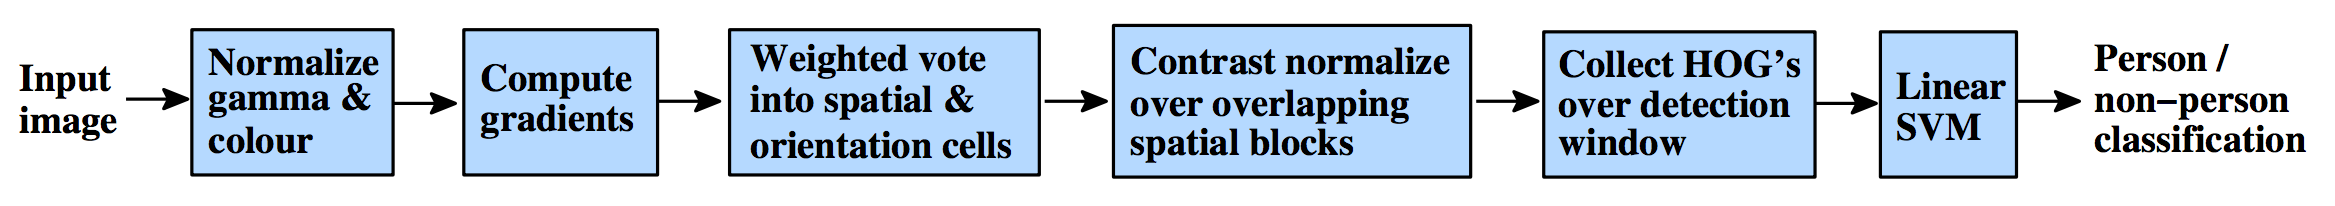
\includegraphics[width=1\linewidth]{pics/feature extraction chain.png} 
	\caption{Ablauf der Klassifizierung von Bildmerkmalen
	\cite{dalal:inria-00548512}}\label{fig:grundlagen_feature_extraction_chain}\end{figure}

Die wichtigsten Bestandteile werde ich im Folgenden erklären.

\subsection{Gradienten-Vektoren}

Wie der Name zu erkennen gibt, betrachtet der \textbf{HOG}-Algorithmus die Gradienten eines Bildes. Beschrieben werden Gradienten durch Vektoren:

$$
\vec{g}=\begin{pmatrix}
	g_x \\
	g_y
\end{pmatrix}
$$

Um die Elemente $g_x$ und $g_y$ zu berechnen, gibt es einige mögliche Filter. Laut $Dalal$ und $Triggs$ \cite[S.5]{dalal:inria-00548512} funktioniert der simple Filter

$$
\vec{x}=\begin{pmatrix}
	-1 & 0 & 1
\end{pmatrix}
$$
bzw.
$$
\vec{y}=\begin{pmatrix}
	-1 \\
	0 \\
	1
\end{pmatrix}
$$
am besten.
Diese Filter werden auf jeden Bildpunkt im Bild angewandt. Somit ergibt sich die Berechnung von $g_x$ und $g_y$ zu:
\begin{equation*}
	g_{x_k}=-x_{k-1}+x_{k+1} \\
	g_{y_k}=-y_{k-1}+y_{k+1}
\end{equation*}

Dabei ist $x_k$ der betrachtete horizontale Bildpunkt und $y_k$ ist der betrachtete vertikale Bildpunkt.
Jedoch aufgepasst, man muss beachten, dass bei einem Farbbild $g_x$ und $g_y$ für jeden Farbkanal berechnet werden müssen. Zusätzlich verhält sich die Berechnung am Rand des Bildes etwas anders.
Wie in der Abbildung ... dargestellt, wird der Wert des Bildpunktes am Rand für die Berechnung einfach wiederholt.

\begin{table}[h!]
\centering
\caption{ANSTATT TABELL, ZEICHNEN!!!Randverhalten!!!}
\label{fig:randverhalten}
\begin{tabular}{c|
>{\columncolor[HTML]{FFFE65}}c |
>{\columncolor[HTML]{FFFE65}}c |
>{\columncolor[HTML]{FFFE65}}c |c}
\cline{2-4}
                                                  & \cellcolor[HTML]{C0C0C0}56 & \cellcolor[HTML]{C0C0C0}... & \cellcolor[HTML]{C0C0C0}98 &                                                  \\ \hline
\multicolumn{1}{|c|}{\cellcolor[HTML]{C0C0C0}56}  & 56                         & ...                         & 98                         & \multicolumn{1}{c|}{\cellcolor[HTML]{C0C0C0}98}  \\ \hline
\multicolumn{1}{|c|}{\cellcolor[HTML]{C0C0C0}...} & ...                        & ...                         & ...                        & \multicolumn{1}{c|}{\cellcolor[HTML]{C0C0C0}...} \\ \hline
\multicolumn{1}{|c|}{\cellcolor[HTML]{C0C0C0}67}  & 67                         & ...                         & 34                         & \multicolumn{1}{c|}{\cellcolor[HTML]{C0C0C0}34}  \\ \hline
                                                  & \cellcolor[HTML]{C0C0C0}67 & \cellcolor[HTML]{C0C0C0}... & \cellcolor[HTML]{C0C0C0}34 &                                                  \\ \cline{2-4}
\end{tabular}
\end{table}

Um nun Histogramme zu erstellen benötigt man für den HOG-Algorithmus zwei Werte. Einmal die Magnitude des Gradienten und dessen Orientierung.
Die Magnitude wird nach dem Satz von Pythagoras durch:
$$ \lvert G \rvert=\sqrt{g_{x_k}^{2}+g_{y_k}^{2}} $$
berechnet und die Orientierung durch:
$$ \theta=\arctan\frac{g_{x_k}}{g_{y_k}} $$.
Die Histogramme entstehen nun durch gewichtetes $binning$ (die Gruppierung zu Intervalle). 

\section{Support Vector Machine}
\label{sec:grundlagensvm}

\section{Tensilica Xtensa LX5}
\label{sec:grundlagenlx5}

\section{Tensilica Instruction Extension}
\label{sec:grundlagentie}

\section{Assembler}
\label{sec:grundlagenassembler}				
\clearpage
\newpage
%
\chapter{Implementierung}
\label{chap:implementierung}

\section{Blaaa}
\label{sec:XXXXXXXXX}

\clearpage
\newpage
%
\chapter{Verifikation und Evaluation}
\label{chap:veriundeval}

Implemented techniques/designs/hardware/software need some sort of validation regarding propriety and performance. The way chosen to establish the correct functionality and/or performance have to be described and justified regarding their suitability.

\section{Verifikation}
\label{sec:verifikation}

Lorem ipsum dolor sit amet, consectetuer adipiscing elit. Aenean commodo ligula eget dolor. Aenean massa. Cum sociis natoque penatibus et magnis dis parturient montes, nascetur ridiculus mus. Donec quam felis, ultricies nec, pellentesque eu, pretium quis, sem. Nulla consequat massa quis enim. Donec pede justo, fringilla vel, aliquet nec, vulputate eget, arcu. In enim justo, rhoncus ut, imperdiet a, venenatis vitae, justo. Nullam dictum felis eu pede mollis pretium. Integer tincidunt. Cras dapibus. Vivamus elementum semper nisi. Aenean vulputate eleifend tellus. Aenean leo ligula, porttitor eu, consequat vitae, eleifend ac, enim.

\section{Evaluation}
\label{sec:evaluation}
\clearpage
\newpage
%
\chapter{Fazit}
\label{chap:fazit}

This chapter contains concluding remarks whether the desired results could be met or why this wasn't the case.
Furthermore future optimizations can be documented here.

\section{Fazit}
\label{sec:conclusion}

Lorem ipsum dolor sit amet, consectetuer adipiscing elit. Aenean commodo ligula eget dolor. Aenean massa. Cum sociis natoque penatibus et magnis dis parturient montes, nascetur ridiculus mus. Donec quam felis, ultricies nec, pellentesque eu, pretium quis, sem. Nulla consequat massa quis enim. Donec pede justo, fringilla vel, aliquet nec, vulputate eget, arcu. In enim justo, rhoncus ut, imperdiet a, venenatis vitae, justo. Nullam dictum felis eu pede mollis pretium. Integer tincidunt. Cras dapibus. Vivamus elementum semper nisi. Aenean vulputate eleifend tellus. Aenean leo ligula, porttitor eu, consequat vitae, eleifend ac, enim.
\clearpage
\newpage
%
\setstretch{1.0}	% set line spacing to single

% the appendix environment should be used for the appendix
% since it is not part of the actual thesis and should therefore
% not follow the same numbering scheme as a regular chapter
\begin{appendix}
	\chapter{ANHANG 1}


	\clearpage
	\newpage
\end{appendix}

\setstretch{1.5}	% set line spacing to single

% Bibliographie unter Verwendung von dinnat %%%%%%%%%%%%%%%%%%%%%%%%%%
%\setbibpreamble{Präambel}		% Text vor dem Verzeichnis
\bibliographystyle{gerunsrt}%{dinat}
\bibliography{bib}	% Sie benötigen einen *.bib-Datei
\clearpage
\newpage
%


%\pagestyle{plain}
%\Large
%Erklärung\\[2ex]
%\setstretch{1.2}
%\normalsize
%Ich versichere hiermit, dass ich die vorstehende Arbeit selbständig angefertigt, keine anderen als die angegebenen Hilfsmittel benutzt und sowohl wörtliche, als auch sinngemäß entlehnte Stellen als solche kenntlich gemacht habe. Die Arbeit hat in gleicher oder ähnlicher Form noch keiner anderen Prüfungsbehörde vorgelegen.

%\vspace{3cm}

%\begin{tabularx}{0.97\textwidth}{p{4cm} X p{6cm}}
%	\hrulefill & ~ & Hannover, den \today\\
%	@TODO Hier eigenen Namen eintragen & ~ & ~ \\
%\end{tabularx}


\end{document}%---------------------------------------------
%
%	titel.tex
%
%---------------------------------------------
	%	
	%
\newpage
\thispagestyle{empty}

% Version I DIY w/o titlepage environment
%\begin{figure}[ht]
%	% optional logo
%		
\includegraphics{pics/IMS_LUH.pdf}
%\end{figure}
%	
%\vspace{20pt}
%
%\begin{center}
%	\Huge\sf{Masterarbeit}\\
%	\vspace{40pt}
%  \LARGE\sf{Der aussagekräftige Titel dieser Arbeit}\\
%	\vspace{60pt}
%  \Large{	Leibniz Universität Hannover\\
%					Fakultät für Elektrotechni`k und Informatik\\
%					Institut für Mikroelektronische Systeme\\
%					Fachgebiet Architekturen und Systeme}\\
%	\vspace{100pt}
%  \large{vorgelegt von}\\
%  \vspace{20pt}
%	\Large{B.Sc. XXXXXXXXXXXX\\
%         Matrikelnummer XXXXXXXX}\\
%  \Large{geb. am: XX.XX.XXXX \hspace{10pt}in: XXXXXX}\\
%	\vspace{30pt}
%	\large{Hannover, \today}
%	  
%  \end{center}

% Version II with titlepage environment
\begin{titlepage}
	\begin{figure}[ht]
		% optional logo
			
\includegraphics{pics/IMS_LUH.pdf}
	\end{figure}
	
\vspace{3cm}

\begin{center}
	\Huge\sf{Bachelorarbeit}\\
	\vspace{40pt}
  \LARGE\sf{HOG - Algorithmus Optimierung durch Tensilica Instruction Extensions}\\
	\vspace{60pt}
  \Large{	Leibniz Universität Hannover\\
					Fakultät für Elektrotechnik und Informatik\\
					Institut für Mikroelektronische Systeme\\
					Fachgebiet Architekturen und Systeme}\\
	\vspace{100pt}
  \large{vorgelegt von}\\
  \vspace{20pt}
	\Large{Alexander Gutwein\\
         Matrikelnummer 2874680}\\
  \Large{geb. am: 18.03.1991 \hspace{10pt}in: Omsk}\\
	\vspace{30pt}
	\large{Hannover, \today}
	  
  \end{center}

\end{titlepage}

% Version III with maketitle
%\titlehead{}
%\subject{Masterarbeit}
%\title{Titel der Arbeit}
%\subtitle{Untertitel}
%\author{B.Sc. XXXXX \\ geb.: XX.XX.XXXX in: XXXXXXXXX \\ Matrikelnummer: XXXXXXX}
%\date{\today}
%\publishers{Betreut und herausgegeben von Prof. Dr.-Ing. Holger Blume}
%\extratitle{schmutztitel}
%\uppertitleback{Obiger Titelrückentitel}
%\lowertitleback{Für dieses Beispiel wird keine Haftung übernommen.}
%\dedication{I would like to express that ..... }
%\maketitle

